\section[toc={New Architectures}]{LHTE Architectures: MLP += \\
  CNNs + ViT + ConvNeXt + EfficientNet}

\begin{slidewhite}[\slideopts,toc={CNN}]{SimpleCNN Architecture}
  
  \centerline{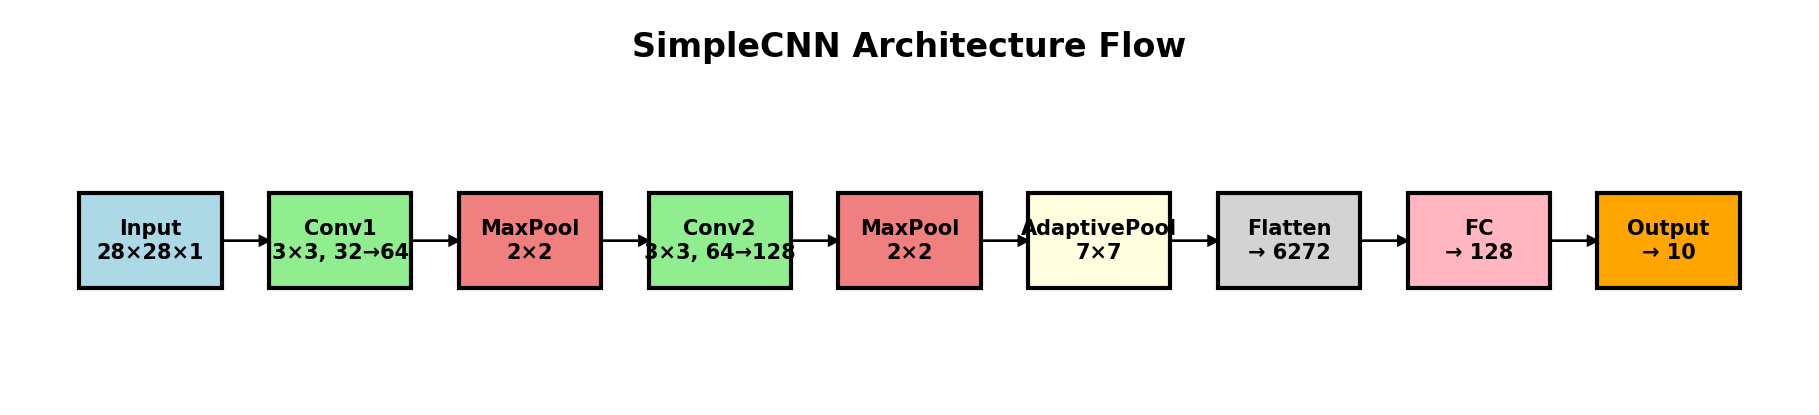
\includegraphics[width=\textwidth]{cnn_architecture.eps}}

  \emph{Convolutional Neural Network for Spatial Feature Extraction}
  
  \begin{itemize}
    \mpitem MNIST and CIFAR-10/100 benchmark examples included, e.g.:
    \begin{itemize}

      \mpitem \emph{Two conv layers:} 3×3 kernels, 32→64 channels, MaxPool, BatchNorm
      
      \mpitem \emph{Adaptive pooling:} 7×7 feature maps → FC classifier with dropout
      
      \mpitem \emph{Parameter variants:} 8K (small), 68K (medium), 421K (large):\\
      \texttt{./configs/mnist\_cnn\_[8k|68k|421k].yaml}
      
      \mpitem \emph{Performance:} CIFAR-10: 85-92\%, CIFAR-100: 55-70\%
    \end{itemize}
    
    \mpitem LHTE adds multihead classification for multi-task learning
  \end{itemize}
  
\end{slidewhite}

\begin{wideslide}[\slideopts,toc={YAML},method=direct]{LHTE Architecture Config Files}
{\footnotesize
\begin{verbatim}
cifar10_cnn_64k.yaml            cifar100_efficientnet_210k.yaml    mnist_efficientnet_22k.yaml
cifar10_convnext_128k.yaml      cifar100_sdn_1m.yaml               mnist_efficientnet_7m.yaml
cifar10_convnext_210k.yaml      cifar100_vit_210k.yaml             mnist_mh_cnn_422k.yaml
cifar10_convnext_64k.yaml       cifar100mh_cnn_64k.yaml            mnist_sdn_68k.yaml
cifar10_efficientnet_210k.yaml  cifar100mh_convnext_210k.yaml      mnist_sdn_8k.yaml
cifar10_mh_cnn_64k.yaml         cifar100mh_efficientnet_210k.yaml  mnist_vit_210k.yaml
cifar10_vit_210k.yaml           cifar100mh_vit_210k.yaml           mnist_vit_38k.yaml
cifar100_cnn_1m_original.yaml   mnist_cnn_421k.yaml                mnist_vit_821k.yaml
cifar100_cnn_1m.yaml            mnist_cnn_68k.yaml                 mnist_vit_995.yaml
cifar100_cnn_64k.yaml           mnist_cnn_8k.yaml                  mnist_vit_pytorch.yaml
cifar100_coarse_cnn_64k.yaml    mnist_convnext_210k.yaml           multihead.yaml
cifar100_convnext_10m.yaml      mnist_convnext_68k.yaml            vimh_cnn_64k_ordinal.yaml
cifar100_convnext_1m.yaml       mnist_convnext_821k.yaml           vimh_cnn_64k_regression.yaml
cifar100_convnext_210k.yaml     mnist_convnext_8k.yaml             vimh_cnn_64k.yaml
\end{verbatim}
}
\textbf{LHT:} \; \texttt{example.yaml}
\end{wideslide}

\begin{slide}[\slideopts,toc={ConvNeXt}]{ConvNeXt-V2 Architecture}
  
  \centerline{\includegraphics[width=\textwidth]{convnext_architecture.eps}}

  \emph{Modern CNN with Global Response Normalization (GRN)}
  
  \begin{itemize}
    \item \emph{Key innovation:} GRN normalizes across spatial/channel dimensions
    
    \item \emph{Architecture:} 7×7 depthwise conv, LayerNorm, 4× MLP with GELU
    
    \item \emph{Sizes:} Tiny (18K), Small (73K), Base (288K), Large (725K)
    
    \item \emph{Best performer:} CIFAR-10: 90-95\%, CIFAR-100: 70-80\%
  \end{itemize}
  
\end{slide}

\begin{slide}[\slideopts,toc={EfficientNet}]{EfficientNet Architecture}
  
  \centerline{\includegraphics[width=1.1\textwidth]{efficientnet_architecture.eps}}

  \emph{Optimized CNN for Mobile and Edge Deployment}
  
  \begin{itemize}
    \item \emph{Compound scaling:} Balances depth, width, and resolution
    
    \item \emph{Mobile-optimized:} Inverted residuals, squeeze-excitation, Swish
    
    \item \emph{Sizes:} 22K (edge), 210K (balanced), 7M (high accuracy)
    
    \item \emph{Performance:} CIFAR-10: 89-94\%, CIFAR-100: 67-77\%
  \end{itemize}
  
\end{slide}

\begin{slide}[\slideopts,toc={ViT}]{Vision Transformer (ViT) Architecture}
  
  \centerline{\includegraphics[width=1.1\textwidth]{vit_architecture.eps}}

  \emph{Attention-Based Learning on Image Patches}
  
  \begin{itemize}
    \item \emph{Image → Patches:} 28×28 → 7×7 patches → token sequence
    
    \item \emph{Self-attention:} Multi-head attention + MLP with GELU
    
    \item \emph{Sizes:} Tiny (38K), Small (210K, MNIST SOTA: 99.5\%), Base (821K)
    
    \item Highly parallelizable, scales with data and compute
  \end{itemize}
  
\end{slide}
